% Gabarit pandoc des corrigés publiés (brut et guidé). Contenu sans marque ni nom de site.
% Compilation : lualatex (latexmk -lualatex).
% Le Markdown reste la source unique : ne pas éditer ce fichier .tex à la main.
\documentclass[11pt,a4paper]{article}

% --- Moteur, polices (Latin Modern) et langue ---------------------------------
\usepackage{iftex}
\ifLuaTeX\else\errmessage{Ce document se compile avec lualatex}\fi
\usepackage{amsmath,amssymb,mathtools}
\usepackage{fontspec}
% mathrm=sym : \mathrm prend ses glyphes dans la police mathématique (ℓ, μ, Ω), comme KaTeX.
\usepackage[math-style=TeX,bold-style=TeX,mathrm=sym]{unicode-math}
% Repli pour les glyphes absents de Latin Modern (indices et exposants Unicode,
% flèches, filets des schémas en texte, symboles) : DejaVu, puis Latin Modern Math
% (ℓ, lettres mathématiques Unicode des légendes).
\directlua{
  luaotfload.add_fallback("repliTexte", {"DejaVuSerif:mode=harf;", "DejaVuSans:mode=harf;", "file:latinmodern-math.otf:mode=harf;"})
  luaotfload.add_fallback("repliMono", {"DejaVuSansMono:mode=harf;", "DejaVuSans:mode=harf;", "file:latinmodern-math.otf:mode=harf;"})
}
\setmainfont{Latin Modern Roman}[RawFeature={fallback=repliTexte}]
\setsansfont{Latin Modern Sans}[RawFeature={fallback=repliTexte}]
\setmonofont{Latin Modern Mono}[RawFeature={fallback=repliMono}]
\setmathfont{Latin Modern Math}
\usepackage[french]{babel}
\frenchsetup{SmallCapsFigTabCaptions=false}

% --- Mise en page --------------------------------------------------------------
\usepackage[a4paper,margin=2.2cm,headheight=14pt,footskip=1.2cm]{geometry}
\usepackage{microtype}
\setlength{\emergencystretch}{4em}
\tolerance=1500
\setlength{\parindent}{0pt}
\setlength{\parskip}{0.55\baselineskip plus 2pt minus 1pt}
\usepackage{xcolor}
% Gris nommés : babel-french rend « ! » actif dans le document.
\definecolor{gris2}{gray}{0.98}
\definecolor{gris3}{gray}{0.97}
\definecolor{gris5}{gray}{0.95}
\definecolor{gris35}{gray}{0.65}
\definecolor{gris40}{gray}{0.60}
\definecolor{gris45}{gray}{0.55}
\definecolor{gris50}{gray}{0.50}
\definecolor{gris55}{gray}{0.45}
\definecolor{gris60}{gray}{0.40}
\definecolor{gris65}{gray}{0.35}
\definecolor{gris70}{gray}{0.30}
\definecolor{gris80}{gray}{0.20}
\definecolor{gris85}{gray}{0.15}
\usepackage{graphicx}
\usepackage{float}
\usepackage{caption}
\captionsetup{font=small,labelformat=empty,justification=centering}
\usepackage{booktabs,longtable,array,multirow,calc}
\usepackage{siunitx}
\sisetup{locale=FR}
\usepackage[version=4]{mhchem}
\usepackage{listings}
\usepackage{fancyhdr}
\usepackage{lastpage}
\usepackage[most]{tcolorbox}
\usepackage{enumitem}
\setlist{nosep,leftmargin=*,topsep=2pt}
\usepackage[hidelinks,unicode]{hyperref}
\usepackage{bookmark}
\hypersetup{pdftitle={Mines-Ponts MP — Maths 2 2026},pdfauthor={Rédigé par IA},pdfcreator={LaTeX},pdfsubject={Corrigé brut}}
\usepackage{xurl}

% --- Pandoc : listes, tableaux, figures ----------------------------------------
\providecommand{\passthrough}[1]{#1}
\providecommand{\tightlist}{\setlength{\itemsep}{0pt}\setlength{\parskip}{0pt}}

\makeatletter
\def\maxwidth{\ifdim\Gin@nat@width>\linewidth\linewidth\else\Gin@nat@width\fi}
\def\maxheight{\ifdim\Gin@nat@height>0.55\textheight 0.55\textheight\else\Gin@nat@height\fi}
\makeatother
\setkeys{Gin}{width=\maxwidth,height=\maxheight,keepaspectratio}
\setcounter{secnumdepth}{-\maxdimen}
\providecommand{\pandocbounded}[1]{#1}

% --- Code (listings) -----------------------------------------------------------
\lstset{
  basicstyle=\ttfamily\small,
  columns=fullflexible,
  keepspaces=true,
  breaklines=true,
  breakatwhitespace=false,
  postbreak=\mbox{\textcolor{gris50}{$\hookrightarrow$}\space},
  frame=single,
  rulecolor=\color{gris35},
  framesep=4pt,
  xleftmargin=5pt,xrightmargin=5pt,
  backgroundcolor=\color{gris3},
  keywordstyle=\bfseries,
  commentstyle=\color{gris65},
  stringstyle=\color{gris80},
  showstringspaces=false,
  tabsize=4,
  extendedchars=true,
  aboveskip=6pt,belowskip=6pt,
}

% --- Macros des corrigés (KaTeX ↔ LaTeX) ---------------------------------------
% Les corrigés sont écrits pour KaTeX : on définit ici ce que KaTeX connaît et
% que LaTeX n'a pas, sans jamais retoucher le Markdown.
\providecommand{\R}{\mathbb{R}}
\providecommand{\N}{\mathbb{N}}
\providecommand{\Z}{\mathbb{Z}}
\providecommand{\Q}{\mathbb{Q}}
\providecommand{\C}{\mathbb{C}}
\providecommand{\dd}{\mathrm{d}}
\providecommand{\llbracket}{\lBrack}
\providecommand{\rrbracket}{\rBrack}
\providecommand{\lBrace}{\lbrace}
\providecommand{\rBrace}{\rbrace}
\providecommand{\Box}{\square}
\providecommand{\Diamond}{\lozenge}
\providecommand{\varnothing}{\emptyset}
\providecommand{\argmax}{\operatorname*{arg\,max}}
\providecommand{\argmin}{\operatorname*{arg\,min}}
\renewcommand{\leq}{\leqslant}
\renewcommand{\geq}{\geqslant}

% Équation hors texte : réduite à la largeur de la ligne si elle déborde.
\newsavebox{\boiteequation}
\newcommand{\equationajustee}[1]{%
  \sbox{\boiteequation}{$\displaystyle #1$}%
  \ifdim\wd\boiteequation>\linewidth
    \[\resizebox{\linewidth}{!}{\usebox{\boiteequation}}\]%
  \else
    \[#1\]%
  \fi}

% --- Encadrés pédagogiques (sobres, lisibles en noir et blanc) -----------------
\tcbset{
  encadre/.style={
    enhanced,breakable,sharp corners,
    colback=white,colframe=gris55,
    boxrule=0.4pt,leftrule=2.2pt,
    left=6pt,right=6pt,top=3pt,bottom=3pt,
    before skip=6pt,after skip=6pt,
    fonttitle=\bfseries\small,coltitle=black,
    attach title to upper,after title={\quad},
    parbox=false,
  }
}
\newtcolorbox{indication}[1]{encadre,colframe=gris45,colback=gris2,title={Indication~#1}}
\newtcolorbox{methode}{encadre,colframe=gris70,title={Méthode}}
\newtcolorbox{piege}{encadre,colframe=gris85,boxrule=0.8pt,leftrule=2.2pt,title={Piège}}
\newtcolorbox{jury}{encadre,colframe=gris60,colback=gris5,title={Jury}}
\newtcolorbox{encadrenote}{encadre,colframe=gris40}

% --- Titres de section ---------------------------------------------------------
\usepackage{titlesec}
\titleformat{\section}{\Large\bfseries}{}{0pt}{}
\titleformat{\subsection}{\large\bfseries}{}{0pt}{}
\titleformat{\subsubsection}{\normalsize\bfseries}{}{0pt}{}
\titlespacing*{\section}{0pt}{14pt plus 4pt minus 2pt}{6pt}
\titlespacing*{\subsection}{0pt}{10pt plus 3pt minus 2pt}{4pt}
\titlespacing*{\subsubsection}{0pt}{8pt plus 2pt minus 2pt}{2pt}

% --- En-tête et pied de page ---------------------------------------------------
\pagestyle{fancy}
\fancyhf{}
\fancyhead[L]{\small\textsc{Corrigé brut} · Mines-Ponts MP}
\fancyhead[R]{\small Maths 2 2026}
\fancyfoot[L]{\footnotesize Corrigé rédigé par IA, non officiel}
\fancyfoot[R]{\footnotesize \thepage\,/\,\pageref*{LastPage}}
\renewcommand{\headrulewidth}{0.4pt}
\renewcommand{\footrulewidth}{0pt}
\fancypagestyle{plain}{\fancyhf{}\fancyfoot[R]{\footnotesize \thepage\,/\,\pageref*{LastPage}}\fancyfoot[L]{\footnotesize Corrigé rédigé par IA, non officiel}\renewcommand{\headrulewidth}{0pt}}

\begin{document}
\thispagestyle{plain}
\begin{center}
  {\small\scshape Corrigé brut}\par\smallskip
  {\LARGE\bfseries Mines-Ponts MP — Maths 2 2026\par}\medskip
  {\large Mines-Ponts · MP · Maths 2 · 2026\par}
\end{center}
\vspace{2pt}\hrule\vspace{8pt}

\emph{Corrigé rédigé par IA, non officiel. Signalez toute erreur.}

\textbf{Autour de \({\mathrm{O}}_n(\mathbb{R})\) et \({\mathrm{SL}}_n(\mathbb{R})\).} Durée 4 h, calculatrice et tout dispositif électronique interdits. 30 questions.

\textbf{Conventions.} \(n\ge 2\), \(E={\mathbb{R}}^n\) muni du produit scalaire canonique et de la norme euclidienne \(\|\cdot\|\). On munit \({\mathcal{M}}_n(\mathbb{R})\) du produit scalaire et de la norme associée :

\equationajustee{\begin{aligned}\langle A,B\rangle&=\operatorname{tr}(A^\top B)=\sum_{i,j}a_{ij}b_{ij},\\\|A\|&=\sqrt{\langle A,A\rangle},\end{aligned}}

de sorte que \(g(M)=\|M\|^2\) et \(\|A^\top\|=\|A\|\). Par l'inégalité de Cauchy-Schwarz appliquée à chaque coefficient \((AB)_{ij}=\sum_k a_{ik}b_{kj}\), on a \(\|AB\|\le\|A\|\,\|B\|\).

De même, \(\|AX\|\le\|A\|\,\|X\|\) pour \(X\in{\mathbb{C}}^n\), muni de la norme hermitienne canonique \(\|X\|^2=\sum|x_k|^2\), car la majoration \(|\sum_k a_{ik}x_k|^2\le(\sum_k a_{ik}^2)(\sum_k|x_k|^2)\) reste valable. On note \({\mathcal{A}}_n(\mathbb{R})\) l'ensemble des matrices antisymétriques.

\begin{center}\rule{0.5\linewidth}{0.5pt}\end{center}

\hypertarget{i.-quelques-propriuxe9tuxe9s-de-mathrmo_nmathbbr}{%
\section{\texorpdfstring{I. Quelques propriétés de \({\mathrm{O}}_n(\mathbb{R})\)}{I. Quelques propriétés de \{\textbackslash mathrm\{O\}\}\_n(\textbackslash mathbb\{R\})}}\label{i.-quelques-propriuxe9tuxe9s-de-mathrmo_nmathbbr}}

\hypertarget{question-1}{%
\subsection{Question 1}\label{question-1}}

Le polynôme caractéristique est \(\chi_{R_\theta}=X^2-2\cos(\theta)X+1\), de discriminant \(4\cos^2\theta-4=-4\sin^2\theta\).

\begin{itemize}
\item
  Si \(\sin\theta=0\) (\(\theta\in\pi\mathbb{Z}\)) : \(R_\theta=\cos(\theta)I_2=\pm I_2\) est diagonale, donc diagonalisable sur \(\mathbb{R}\) et sur \(\mathbb{C}\).
\item
  Si \(\sin\theta\neq0\) : le discriminant est \(<0\), donc \(\chi_{R_\theta}\) n'a pas de racine réelle et \(R_\theta\) n'a aucune valeur propre réelle.

  Une matrice diagonalisable sur \(\mathbb{R}\) est semblable à une matrice diagonale réelle dont les coefficients sont des valeurs propres réelles : \(R_\theta\) n'est donc pas diagonalisable sur \(\mathbb{R}\).

  Sur \(\mathbb{C}\), \(\chi_{R_\theta}\) a les deux racines \(e^{i\theta}\) et \(e^{-i\theta}\) (somme \(2\cos\theta\), produit \(1\)).

  Elles sont distinctes puisque \(e^{i\theta}-e^{-i\theta}=2i\sin\theta\neq0\). Une matrice de taille 2 ayant deux valeurs propres distinctes est diagonalisable : \(R_\theta\) est semblable à \(\operatorname{diag}(e^{i\theta},e^{-i\theta})\).
\end{itemize}

\textbf{\(R_\theta\) est toujours diagonalisable sur \(\mathbb{C}\) ; elle est diagonalisable sur \(\mathbb{R}\) si et seulement si \(\theta\in\pi\mathbb{Z}\), c'est-à-dire \(R_\theta=\pm I_2\).}

\hypertarget{question-2}{%
\subsection{Question 2}\label{question-2}}

\emph{Inclusion \(\supset\).} Par le calcul direct,

\equationajustee{R_\theta^\top R_\theta=\begin{pmatrix}\cos^2\theta+\sin^2\theta&0\\0&\sin^2\theta+\cos^2\theta\end{pmatrix}=I_2,}

et \(\det R_\theta=\cos^2\theta+\sin^2\theta=1\), donc \(R_\theta\in{\mathrm{SO}}_2(\mathbb{R})\).

\emph{Inclusion \(\subset\).} Soit \(M=\begin{pmatrix}a&b\\c&d\end{pmatrix}\in{\mathrm{SO}}_2(\mathbb{R})\), de colonnes \(C_1=(a,c)\) et \(C_2=(b,d)\). La relation \(M^\top M=I_2\) signifie que \((C_1,C_2)\) est orthonormée :

\equationajustee{\begin{aligned}a^2+c^2&=1,\\b^2+d^2&=1,\\ab+cd&=0.\end{aligned}}

Comme \(a^2+c^2=1\), il existe \(\theta\in\mathbb{R}\) tel que \(a=\cos\theta\) et \(c=\sin\theta\) (paramétrage du cercle unité).

Le vecteur \(C_2\) appartient à \(C_1^\perp\), droite de \({\mathbb{R}}^2\) dirigée par le vecteur unitaire \(u=(-\sin\theta,\cos\theta)\). Étant unitaire, \(C_2=\pm u\).

Si \(C_2=-u\), alors \(M=\begin{pmatrix}\cos\theta&\sin\theta\\\sin\theta&-\cos\theta\end{pmatrix}\) et \(\det M=-1\), exclu. Donc \(C_2=u\) et \(M=R_\theta\).

\begin{figure}[H]
\centering
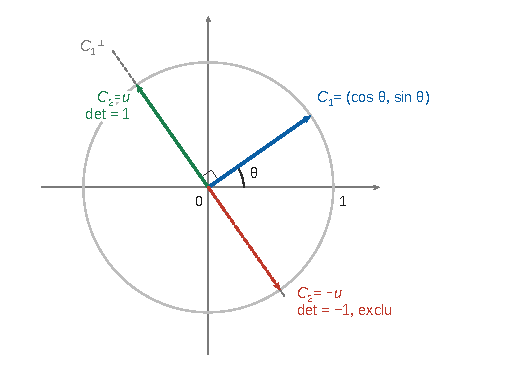
\includegraphics{figures/q2-colonnes-so2.pdf}
\caption*{Figure 1 --- Les deux vecteurs unitaires de C₁⊥ : C₂ = u convient, C₂ =
−u donne det M = −1}
\end{figure}

\equationajustee{\boxed{{\mathrm{SO}}_2(\mathbb{R})=\{R_\theta,\ \theta\in\mathbb{R}\}}}

\hypertarget{question-3}{%
\subsection{Question 3}\label{question-3}}

\emph{Compacité.} L'application \(f:M\mapsto M^\top M\) est continue, car ses coefficients sont polynomiaux en ceux de \(M\). Donc \({\mathrm{O}}_n(\mathbb{R})=f^{-1}(\{I_n\})\) est fermé, image réciproque d'un fermé par une application continue.

Pour \(M\in{\mathrm{O}}_n(\mathbb{R})\), \(\|M\|^2=\operatorname{tr}(M^\top M)=\operatorname{tr}(I_n)=n\), donc \(\|M\|=\sqrt n\) : \({\mathrm{O}}_n(\mathbb{R})\) est borné. Fermé et borné dans l'espace \({\mathcal{M}}_n(\mathbb{R})\) de dimension finie, \textbf{\({\mathrm{O}}_n(\mathbb{R})\) est compact}.

\emph{Non-connexité par arcs.} Pour \(M\in{\mathrm{O}}_n(\mathbb{R})\), \((\det M)^2=\det(M^\top M)=1\), donc \(\det M\in\{-1,1\}\). Les deux valeurs sont atteintes :

\begin{itemize}
\tightlist
\item
  \(I_n\in{\mathrm{O}}_n(\mathbb{R})\), de déterminant \(1\) ;
\item
  \(S=\operatorname{diag}(-1,\allowbreak 1,\allowbreak \dots,\allowbreak 1)\in{\mathrm{O}}_n(\mathbb{R})\), car \(S^\top S=S^2=I_n\), de déterminant \(-1\).
\end{itemize}

S'il existait un chemin continu \(\gamma:[0,1]\to{\mathrm{O}}_n(\mathbb{R})\) de \(I_n\) à \(S\), la fonction réelle continue \(\det\circ\gamma\) passerait de \(1\) à \(-1\).

Par le théorème des valeurs intermédiaires, elle s'annulerait, ce qui contredit \(\det({\mathrm{O}}_n(\mathbb{R}))\subset\{-1,1\}\). \textbf{\({\mathrm{O}}_n(\mathbb{R})\) n'est pas connexe par arcs.}

\hypertarget{question-4}{%
\subsection{Question 4}\label{question-4}}

Il suffit de joindre tout \(M\in{\mathrm{SO}}_n(\mathbb{R})\) à \(I_n\) par un chemin continu à valeurs dans \({\mathrm{SO}}_n(\mathbb{R})\) : deux éléments quelconques sont alors reliés en passant par \(I_n\) (concaténation de chemins). On le montre par récurrence sur \(n\ge2\).

\emph{Cas \(n=2\).} Par la question 2, \(M=R_\theta\).

Le chemin \(t\mapsto R_{(1-t)\theta}\), \(t\in[0,1]\), est continu, à valeurs dans \({\mathrm{SO}}_2(\mathbb{R})\), et va de \(M\) à \(I_2\).

\emph{Hérédité.} Soit \(n\ge3\), la propriété étant acquise en dimension \(n-1\). Soit \(M\in{\mathrm{SO}}_n(\mathbb{R})\) et \(y=Me_1\), unitaire.

\begin{figure}[H]
\centering
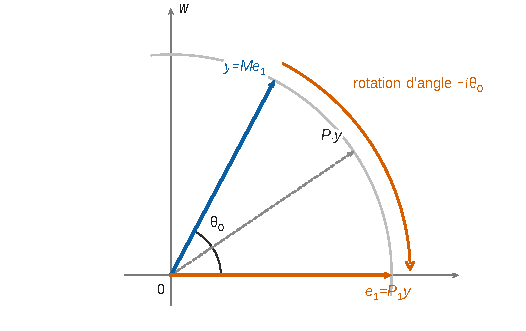
\includegraphics{figures/q4-rotation-plan.pdf}
\caption*{Figure 2 --- Dans le plan Vect(e₁, w), la rotation Pₜ d'angle −tθ₀
ramène continûment y = Me₁ sur e₁}
\end{figure}

\begin{enumerate}
\def\labelenumi{\arabic{enumi}.}
\item
  \emph{On ramène \(y\) sur \(e_1\).} Choisissons un vecteur unitaire \(w\perp e_1\) et \(\theta_0\in[0,\pi]\) tels que \(y=\cos(\theta_0)e_1+\sin(\theta_0)w\).

  \begin{itemize}
  \tightlist
  \item
    Si \(y\neq\pm e_1\), on prend \(\cos\theta_0=\langle y,e_1\rangle\), \(\sin\theta_0=\|y-\langle y,e_1\rangle e_1\|\) et
    \equationajustee{w=\dfrac{y-\langle y,e_1\rangle e_1}{\|y-\langle y,e_1\rangle e_1\|}.}
  \item
    Si \(y=e_1\), \(\theta_0=0\) et \(w\) est quelconque ; si \(y=-e_1\), \(\theta_0=\pi\) et \(w\) est quelconque.
  \end{itemize}

  Complétons \((e_1,w)\) en une base orthonormée de \(E\), de matrice de passage \(U\in{\mathrm{O}}_n(\mathbb{R})\), et posons, pour \(t\in[0,1]\),
  \equationajustee{P_t=U\begin{pmatrix}R_{-t\theta_0}&0\\0&I_{n-2}\end{pmatrix}U^{-1}.}
  \(P_t\) est orthogonale (produit de matrices orthogonales), de déterminant \(\det R_{-t\theta_0}=1\). L'application \(t\mapsto P_t\) est continue et \(P_0=I_n\).

  Comme \(U^{-1}y=(\cos\theta_0,\sin\theta_0,0,\dots,0)^\top\) et \(R_{-\theta_0}(\cos\theta_0,\sin\theta_0)^\top=(1,0)^\top\), on a \(P_1y=e_1\).

  Le chemin \(t\mapsto P_tM\) est continu dans \({\mathrm{SO}}_n(\mathbb{R})\) et joint \(M\) à \(M'=P_1M\), qui vérifie \(M'e_1=e_1\).
\item
  \emph{On descend en dimension \(n-1\).} \(M'\) fixe \(e_1\). Pour \(x\perp e_1\),
  \equationajustee{\begin{aligned}\langle M'x,e_1\rangle&=\langle M'x,M'e_1\rangle\\&=\langle x,e_1\rangle=0,\end{aligned}}
  donc \(M'\) stabilise \(e_1^\perp=\operatorname{Vect}(e_2,\dots,e_n)\) et \(M'=\begin{pmatrix}1&0\\0&M''\end{pmatrix}\), avec \(M''^\top M''=I_{n-1}\) et \(\det M''=\det M'=1\).

  Par hypothèse de récurrence, un chemin \(\Gamma\) joint \(M''\) à \(I_{n-1}\) dans \({\mathrm{SO}}_{n-1}(\mathbb{R})\).

  Le chemin \(t\mapsto\begin{pmatrix}1&0\\0&\Gamma(t)\end{pmatrix}\) joint alors \(M'\) à \(I_n\) dans \({\mathrm{SO}}_n(\mathbb{R})\).
\end{enumerate}

Par concaténation, \(M\) est joint à \(I_n\) dans \({\mathrm{SO}}_n(\mathbb{R})\). \textbf{\({\mathrm{SO}}_n(\mathbb{R})\) est connexe par arcs.}

\hypertarget{question-5}{%
\subsection{Question 5}\label{question-5}}

Soit \(H\) un sous-groupe de \({\mathrm{O}}_n(\mathbb{R})\) contenant \({\mathrm{SO}}_n(\mathbb{R})\). Si \(H\subset{\mathrm{SO}}_n(\mathbb{R})\), alors \(H={\mathrm{SO}}_n(\mathbb{R})\).

Sinon, il existe \(A\in H\) avec \(\det A=-1\). Soit \(B\in{\mathrm{O}}_n(\mathbb{R})\).

\begin{itemize}
\tightlist
\item
  Si \(\det B=1\), alors \(B\in{\mathrm{SO}}_n(\mathbb{R})\subset H\).
\item
  Si \(\det B=-1\), alors \(A^{-1}B\in{\mathrm{O}}_n(\mathbb{R})\) et \(\det(A^{-1}B)=1\), donc \(A^{-1}B\in{\mathrm{SO}}_n(\mathbb{R})\subset H\), puis \(B=A(A^{-1}B)\in H\).
\end{itemize}

Ainsi \({\mathrm{O}}_n(\mathbb{R})\subset H\subset{\mathrm{O}}_n(\mathbb{R})\).

\textbf{\(H={\mathrm{SO}}_n(\mathbb{R})\) ou \(H={\mathrm{O}}_n(\mathbb{R})\).}

\hypertarget{question-6}{%
\subsection{Question 6}\label{question-6}}

\emph{\({\mathrm{GL}}_2\).} On a \(\det Z_2=U-V\) avec \(U=Y_{1,1}Y_{2,2}\) et \(V=Y_{1,2}Y_{2,1}\). Ces variables sont à valeurs dans \(\{0,1\}\) et indépendantes (fonctions de familles disjointes de variables indépendantes).

Par indépendance, \(P(U=1)=P(V=1)=p^2\). Alors \(Z_2\in{\mathrm{GL}}_2(\mathbb{R})\iff U\neq V\), d'où

\equationajustee{\begin{aligned}P(Z_2\in{\mathrm{GL}}_2(\mathbb{R}))&=P(U=1)P(V=0)+P(U=0)P(V=1)\\&=2p^2(1-p^2).\end{aligned}}

\equationajustee{\boxed{P(Z_2\in{\mathrm{GL}}_2(\mathbb{R}))=2p^2(1-p^2)}}

\emph{\({\mathrm{O}}_n\).} Soit \(A\) à coefficients dans \(\{0,1\}\) et orthogonale.

Chaque colonne \(C_j\) vérifie \(\|C_j\|^2=\sum_i a_{ij}^2=\sum_i a_{ij}=1\) : elle contient exactement un coefficient \(1\), en une ligne notée \(\sigma(j)\).

Pour \(j\neq j'\), \(\langle C_j,C_{j'}\rangle=\sum_i a_{ij}a_{ij'}=0\) avec des termes positifs, donc \(\sigma(j)\neq\sigma(j')\). Ainsi \(\sigma\) est injective, donc bijective, et \(A\) est la matrice de permutation \(P_\sigma\). Réciproquement, toute matrice de permutation est orthogonale (ses colonnes forment une permutation de la base canonique).

Les événements \(\{Z_n=P_\sigma\}\) sont deux à deux incompatibles. Par indépendance des \(n^2\) coefficients, \(P(Z_n=P_\sigma)=p^n(1-p)^{n^2-n}\). Donc

\equationajustee{\boxed{P(Z_n\in{\mathrm{O}}_n(\mathbb{R}))=n!\,p^n(1-p)^{n^2-n}.}}

\emph{\({\mathrm{SO}}_n\).} On a \(\det P_\sigma=\varepsilon(\sigma)\), donc \(P_\sigma\in{\mathrm{SO}}_n(\mathbb{R})\) si et seulement si \(\sigma\) est paire.

Pour \(n\ge2\), la signature est un morphisme surjectif de \({\mathfrak{S}}_n\) sur \(\{-1,1\}\), de noyau \({\mathfrak{A}}_n\) ; donc \({\mathfrak{A}}_n\) a \(n!/2\) éléments, et

\equationajustee{\boxed{P(Z_n\in{\mathrm{SO}}_n(\mathbb{R}))=\frac{n!}{2}\,p^n(1-p)^{n^2-n}.}}

\hypertarget{question-7}{%
\subsection{Question 7}\label{question-7}}

Pour \(u\in E\) non nul, la réflexion d'hyperplan \(u^\perp\) est

\equationajustee{s_u:v\mapsto v-2\dfrac{\langle v,u\rangle}{\|u\|^2}u ;}

sa matrice dans la base canonique est une matrice de réflexion (orthogonale, de déterminant \(-1\)).

\begin{itemize}
\item
  Si \(x\neq y\), posons \(u=x-y\neq0\). Comme \(\|x\|=\|y\|\),
  \equationajustee{\begin{aligned}\|u\|^2&=\|x\|^2-2\langle x,y\rangle+\|y\|^2\\&=2(\|x\|^2-\langle x,y\rangle)\\&=2\langle x,u\rangle,\end{aligned}}
  donc \(s_u(x)=x-u=y\). Géométriquement : \(\langle x+y,x-y\rangle=\|x\|^2-\|y\|^2=0\), donc \(x+y\in u^\perp\) est fixé par \(s_u\) et \(x-y\) est changé en son opposé.

  Avec \(x=\frac12(x+y)+\frac12(x-y)\), on retrouve \(s_u(x)=\frac12(x+y)-\frac12(x-y)=y\).
\item
  Si \(x=y\), comme \(n\ge2\), l'hyperplan \(x^\perp\) est de dimension au moins \(n-1\ge1\).

  Il existe donc \(u\neq0\) orthogonal à \(x\), et alors \(s_u(x)=x=y\).

  L'identité, de déterminant \(1\), n'est pas une réflexion : ce cas demande bien une réflexion d'hyperplan contenant \(x\).
\end{itemize}

\begin{figure}[H]
\centering
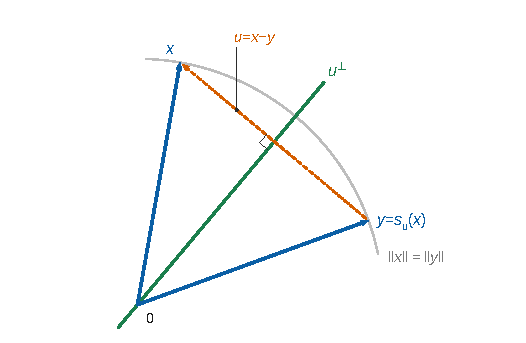
\includegraphics{figures/q7-reflexion.pdf}
\caption*{Figure 3 --- Avec u = x − y, l'hyperplan u⊥ est la médiatrice du segment
joignant x à y : la réflexion s\_u envoie x sur y}
\end{figure}

\textbf{Dans les deux cas, la matrice \(A\) de \(s_u\) est une matrice de réflexion telle que \(Ax=y\).}

\hypertarget{question-8}{%
\subsection{Question 8}\label{question-8}}

Soient \(G\in\mathcal{G}\), \(x\) unitaire et \(\lambda=\|Gx\|\) ; \(\lambda>0\) car \(G\) est inversible et \(x\neq0\).

\emph{Cas \(p=1\).} On a \(\|\lambda x\|=\lambda=\|Gx\|\). Par la question 7, il existe une matrice de réflexion \(A\) avec \(A(Gx)=\lambda x\).

Comme \(A\in{\mathrm{O}}_n(\mathbb{R})\subset\mathcal{G}\) et que \(\mathcal{G}\) est un groupe, \(G_1:=AG\in\mathcal{G}\) et \(G_1x=\lambda x\).

\emph{Cas général.} Posons \(G_p=G_1^{\,p}\in\mathcal{G}\) pour \(p\in\mathbb{Z}\) (stabilité d'un groupe par puissances entières). Par récurrence, \(G_1^{\,p}x=\lambda^px\) pour \(p\in\mathbb{N}\).

De \(G_1x=\lambda x\) et \(\lambda\neq0\), on tire \(G_1^{-1}x=\lambda^{-1}x\), puis \(G_1^{-p}x=\lambda^{-p}x\) pour \(p\in\mathbb{N}\). Ainsi

\equationajustee{\boxed{\forall p\in\mathbb{Z},\ G_p\in\mathcal{G}\ \text{ et }\ G_px=\|Gx\|^p\,x.}}

\hypertarget{question-9}{%
\subsection{Question 9}\label{question-9}}

\(\mathcal{G}\) est compact donc borné : il existe \(C>0\) tel que \(\|H\|\le C\) pour tout \(H\in\mathcal{G}\).

Soient \(G\in\mathcal{G}\), \(x\) unitaire et \(\lambda=\|Gx\|>0\). Pour tout \(p\in\mathbb{Z}\), avec \(G_p\) de la question 8,

\equationajustee{\begin{aligned}\lambda^p&=\|G_px\|\\&\le\|G_p\|\,\|x\|\\&\le C.\end{aligned}}

Si \(\lambda>1\), \(\lambda^p\to+\infty\) quand \(p\to+\infty\) ; si \(\lambda<1\), \(\lambda^p\to+\infty\) quand \(p\to-\infty\) : contradiction dans les deux cas.

Donc \(\|Gx\|=1\) pour tout \(x\) unitaire, puis, par homogénéité, \(\|Gv\|=\|v\|\) pour tout \(v\in E\).

Par polarisation, avec \(\langle a,b\rangle=\frac12(\|a+b\|^2-\|a\|^2-\|b\|^2)\), on obtient \(\langle Ga,Gb\rangle=\langle a,b\rangle\), c'est-à-dire \(\langle(G^\top G-I_n)a,b\rangle=0\) pour tous \(a,b\). Avec \(b=(G^\top G-I_n)a\), on obtient \(G^\top G=I_n\).

Donc \(\mathcal{G}\subset{\mathrm{O}}_n(\mathbb{R})\), et l'inclusion réciproque est une hypothèse :

\equationajustee{\boxed{\mathcal{G}={\mathrm{O}}_n(\mathbb{R}).}}

\begin{center}\rule{0.5\linewidth}{0.5pt}\end{center}

\hypertarget{ii.-calcul-diffuxe9rentiel-sur-mathrmo_nmathbbr-et-mathrmsl_nmathbbr}{%
\section{\texorpdfstring{II. Calcul différentiel sur \({\mathrm{O}}_n(\mathbb{R})\) et \({\mathrm{SL}}_n(\mathbb{R})\)}{II. Calcul différentiel sur \{\textbackslash mathrm\{O\}\}\_n(\textbackslash mathbb\{R\}) et \{\textbackslash mathrm\{SL\}\}\_n(\textbackslash mathbb\{R\})}}\label{ii.-calcul-diffuxe9rentiel-sur-mathrmo_nmathbbr-et-mathrmsl_nmathbbr}}

\hypertarget{question-10}{%
\subsection{Question 10}\label{question-10}}

\emph{Classe \({\mathcal{C}}^1\).} Les coordonnées de \(f\) dans la base canonique sont

\equationajustee{\begin{aligned}f(M)_{ij}&=(M^\top M)_{ij}\\&=\sum_{k=1}^n m_{ki}m_{kj},\end{aligned}}

fonctions polynomiales des coefficients de \(M\). Toutes les dérivées partielles existent et sont continues : \textbf{\(f\) est de classe \({\mathcal{C}}^1\)} (et même \({\mathcal{C}}^\infty\)).

\emph{Différentielle.} Pour \(M,H\in{\mathcal{M}}_n(\mathbb{R})\) :

\equationajustee{f(M+H)=f(M)+(M^\top H+H^\top M)+H^\top H.}

L'application \(L_M:H\mapsto M^\top H+H^\top M\) est linéaire : pour \(H,K\) et \(\mu\in\mathbb{R}\), \(L_M(H+\mu K)=L_M(H)+\mu L_M(K)\), par linéarité de la transposition et bilinéarité du produit. Le reste vérifie, par sous-multiplicativité et \(\|H^\top\|=\|H\|\) pour la norme choisie,

\equationajustee{\begin{aligned}\|H^\top H\|&\le\|H^\top\|\,\|H\|\\&=\|H\|^2=o(\|H\|).\end{aligned}}

Donc \(f\) est différentiable en tout \(M\) et

\equationajustee{\boxed{\mathrm{d}f(M)\cdot H=M^\top H+H^\top M.}}

On retrouve le caractère \({\mathcal{C}}^1\) : \(M\mapsto\mathrm{d}f(M)\) est linéaire de \({\mathcal{M}}_n(\mathbb{R})\) dans \(\mathcal{L}({\mathcal{M}}_n(\mathbb{R}))\), espace de dimension finie, donc continue.

\hypertarget{question-11}{%
\subsection{Question 11}\label{question-11}}

Soit \(H\in T\), associé à \(\gamma:\,]-\varepsilon,\allowbreak \varepsilon[\,\to{\mathrm{O}}_n(\mathbb{R})\) dérivable en \(0\), avec \(\gamma(0)=I_n\) et \(\gamma'(0)=H\).

On a \(f\circ\gamma=I_n\) (constante). Comme \(f\) est différentiable en \(I_n\) et \(\gamma\) dérivable en \(0\), la règle de dérivation le long d'un arc donne

\equationajustee{\begin{aligned}0&=(f\circ\gamma)'(0)\\&=\mathrm{d}f(I_n)\cdot H\\&=H+H^\top.\end{aligned}}

\textbf{Donc \(H^\top=-H\) : \(T\subset{\mathcal{A}}_n(\mathbb{R})\).}

\hypertarget{question-12}{%
\subsection{Question 12}\label{question-12}}

\emph{Somme.} Soient \(H,K\in T\), d'arcs \(\gamma_H\) et \(\gamma_K\).

Sur \(]-\varepsilon,\varepsilon[\) avec \(\varepsilon=\min(\varepsilon_H,\varepsilon_K)\), posons \(\gamma=\gamma_H\gamma_K\). Cet arc est à valeurs dans \({\mathrm{O}}_n(\mathbb{R})\) (groupe) et \(\gamma(0)=I_n\).

Le produit matriciel étant bilinéaire, \(\gamma\) est dérivable en \(0\) avec

\equationajustee{\begin{aligned}\gamma'(0)&=\gamma_H'(0)\gamma_K(0)+\gamma_H(0)\gamma_K'(0)\\&=H+K.\end{aligned}}

Donc \textbf{\(H+K\in T\)}.

\emph{Structure d'espace vectoriel.} \(0\in T\) (arc constant égal à \(I_n\)).

Pour \(H\in T\) et \(\lambda\neq0\), l'arc \(\delta(t)=\gamma_H(\lambda t)\), défini sur \(]-\varepsilon/|\lambda|,\varepsilon/|\lambda|[\), est à valeurs dans \({\mathrm{O}}_n(\mathbb{R})\).

Il vérifie \(\delta(0)=I_n\) et il est dérivable en \(0\) de dérivée \(\lambda H\) ; donc \(\lambda H\in T\) (et \(0\cdot H=0\in T\)).

\textbf{\(T\) est un sous-espace vectoriel de \({\mathcal{M}}_n(\mathbb{R})\)}, donc un \(\mathbb{R}\)-espace vectoriel.

\hypertarget{question-13}{%
\subsection{Question 13}\label{question-13}}

Soit \(H\in{\mathcal{A}}_n(\mathbb{R})\) et \(\gamma(t)=\exp(tH)\). Par continuité de la transposition, \(\exp(tH)^\top=\exp(tH^\top)=\exp(-tH)\). Comme \(tH\) et \(-tH\) commutent,

\equationajustee{\begin{aligned}\gamma(t)^\top\gamma(t)&=\exp(-tH)\exp(tH)\\&=\exp(0)=I_n :\end{aligned}}

\(\gamma\) est à valeurs dans \({\mathrm{O}}_n(\mathbb{R})\), et \(\gamma(0)=I_n\). Enfin, pour \(t\neq0\),

\equationajustee{\begin{aligned}\Big\|\frac{\gamma(t)-I_n}{t}-H\Big\|&\le\frac1{|t|}\sum_{k\ge2}\frac{|t|^k\|H\|^k}{k!}\\&=\frac{e^{|t|\|H\|}-1-|t|\|H\|}{|t|}\xrightarrow[t\to0]{}0,\end{aligned}}

donc \(\gamma'(0)=H\) et \(H\in T\). Avec la question 11 :

\equationajustee{\boxed{T={\mathcal{A}}_n(\mathbb{R}).}}

\(T\) est l'ensemble des matrices \(H\in{\mathcal{M}}_n(\mathbb{R})\) telles que \(H^\top=-H\).

\hypertarget{question-14}{%
\subsection{Question 14}\label{question-14}}

Pour \(t>0\), la matrice \(D_t=\operatorname{diag}(t,1/t,1,\dots,1)\) (possible car \(n\ge2\)) vérifie \(\det D_t=1\) et

\equationajustee{g(D_t)=t^2+\frac1{t^2}+(n-2)\xrightarrow[t\to+\infty]{}+\infty.}

\textbf{La restriction de \(g\) à \({\mathrm{SL}}_n(\mathbb{R})\) n'est pas majorée, donc n'a pas de maximum global.}

\hypertarget{question-15}{%
\subsection{Question 15}\label{question-15}}

On a \(g(M)=\sum_{i,j}m_{ij}^2\) et \(\det M=\sum_{\sigma\in{\mathfrak{S}}_n}\varepsilon(\sigma)\prod_i m_{\sigma(i)i}\). Ces fonctions sont polynomiales en les coefficients de \(M\), donc de classe \({\mathcal{C}}^\infty\), en particulier \({\mathcal{C}}^1\).

\emph{Gradient de \(g\).} Comme \(\operatorname{tr}(H^\top M)=\operatorname{tr}(M^\top H)\),

\equationajustee{g(M+H)=g(M)+2\langle M,H\rangle+\|H\|^2,}

et \(\|H\|^2=o(\|H\|)\), donc \(\mathrm{d}g(M)\cdot H=\langle 2M,H\rangle\) :

\equationajustee{\boxed{\nabla g(M)=2M.}}

\emph{Gradient de \(\det\).} Notons \(\Delta_{ik}(M)\) le mineur d'indice \((i,k)\) : c'est le déterminant de la matrice extraite de \(M\) en supprimant la ligne \(i\) et la colonne \(k\).

Le cofacteur est \(\operatorname{Com}(M)_{ik}=(-1)^{i+k}\Delta_{ik}(M)\).

Le développement selon la ligne \(i\) s'écrit

\equationajustee{\det M=\sum_k m_{ik}\operatorname{Com}(M)_{ik}.}

Le cofacteur \(\operatorname{Com}(M)_{ik}\) ne fait intervenir aucun coefficient de la ligne \(i\), donc ne dépend pas de \(m_{ij}\). Par conséquent \(\dfrac{\partial\det}{\partial m_{ij}}(M)=\operatorname{Com}(M)_{ij}\), et, \(\det\) étant \({\mathcal{C}}^1\),

\equationajustee{\begin{aligned}\mathrm{d}\det(M)\cdot H&=\sum_{i,j}\operatorname{Com}(M)_{ij}h_{ij}\\&=\langle\operatorname{Com}(M),H\rangle.\end{aligned}}

\equationajustee{\boxed{\nabla\det(M)=\operatorname{Com}(M).}}

\hypertarget{question-16}{%
\subsection{Question 16}\label{question-16}}

\({\mathrm{SL}}_n(\mathbb{R})\) est l'ensemble des zéros de \(h=\det-1\), de classe \({\mathcal{C}}^1\) sur l'ouvert \({\mathcal{M}}_n(\mathbb{R})\), et \(g\) y est aussi de classe \({\mathcal{C}}^1\) (question 15).

Soit \(M\in{\mathrm{SL}}_n(\mathbb{R})\) où \(g_{|{\mathrm{SL}}_n(\mathbb{R})}\) a un extremum local.

Comme \(M\operatorname{Com}(M)^\top=\det(M)I_n=I_n\), on a \(\operatorname{Com}(M)=(M^{-1})^\top\neq0\), donc \(\mathrm{d}h(M)\neq0\).

Le théorème d'optimisation sous une contrainte s'applique et donne la colinéarité de \(\mathrm{d}g(M)\) et \(\mathrm{d}h(M)\) : il existe \(\mu\in\mathbb{R}\) tel que \(2M=\mu\operatorname{Com}(M)\). Avec \(\lambda=\mu/2\) :

\equationajustee{\boxed{M=\lambda\operatorname{Com}(M),\ \lambda\in\mathbb{R}.}}

Alors \(M=\lambda(M^{-1})^\top\), d'où \(M^\top=\lambda M^{-1}\) et \(M^\top M=\lambda I_n\).

\begin{itemize}
\tightlist
\item
  En prenant la trace : \(n\lambda=\|M\|^2>0\) (car \(M\neq0\)), donc \(\lambda>0\).
\item
  En prenant le déterminant : \(\lambda^n=\det(\lambda I_n)=(\det M)^2=1\).
\end{itemize}

Comme \(\lambda>0\), \(\lambda=1\). Ainsi \(M^\top M=I_n\) et \(\det M=1\), \textbf{donc \(M\in{\mathrm{SO}}_n(\mathbb{R})\)}.

\hypertarget{question-17}{%
\subsection{Question 17}\label{question-17}}

\emph{Existence.} Soit

\equationajustee{\begin{aligned}K&=\{M\in{\mathrm{SL}}_n(\mathbb{R}),\ g(M)\le n\}\\&=\det{}^{-1}(\{1\})\cap g^{-1}(]-\infty,n]).\end{aligned}}

\(K\) est fermé (intersection d'images réciproques de fermés par des applications continues), borné (\(\|M\|^2\le n\)) et non vide (\(I_n\in K\)), donc compact (dimension finie). La fonction continue \(g\) y atteint son minimum en un \(M_0\), avec \(g(M_0)\le g(I_n)=n\).

Pour \(M\in{\mathrm{SL}}_n(\mathbb{R})\setminus K\), \(g(M)>n\ge g(M_0)\). Donc \(g(M_0)\) est le \textbf{minimum global} de \(g\) sur \({\mathrm{SL}}_n(\mathbb{R})\).

\emph{Valeur et points.} Si \(M\) réalise ce minimum, c'est un extremum local de \(g_{|{\mathrm{SL}}_n(\mathbb{R})}\). Donc \(M\in{\mathrm{SO}}_n(\mathbb{R})\) (question 16) et \(g(M)=\operatorname{tr}(I_n)=n\).

Réciproquement, tout \(M\in{\mathrm{SO}}_n(\mathbb{R})\) est dans \({\mathrm{SL}}_n(\mathbb{R})\) et vérifie \(g(M)=n\).

\equationajustee{\boxed{\min_{{\mathrm{SL}}_n(\mathbb{R})}g=n,\ \text{atteint exactement sur }{\mathrm{SO}}_n(\mathbb{R}).}}

\begin{center}\rule{0.5\linewidth}{0.5pt}\end{center}

\hypertarget{iii.-morphismes-continus-de-mathbbu-dans-mathrmgl_nmathbbr}{%
\section{\texorpdfstring{III. Morphismes continus de \(\mathbb{U}\) dans \({\mathrm{GL}}_n(\mathbb{R})\)}{III. Morphismes continus de \textbackslash mathbb\{U\} dans \{\textbackslash mathrm\{GL\}\}\_n(\textbackslash mathbb\{R\})}}\label{iii.-morphismes-continus-de-mathbbu-dans-mathrmgl_nmathbbr}}

\hypertarget{question-18}{%
\subsection{Question 18}\label{question-18}}

\emph{Sous-groupes bornés de \({\mathbb{R}}^*\).} Soit \(H\) un sous-groupe borné et \(x\in H\) ; \(x^k\in H\) pour tout \(k\in\mathbb{Z}\).

Si \(|x|>1\), \(|x|^k\to+\infty\) quand \(k\to+\infty\) ; si \(|x|<1\), \(|x|^{-k}\to+\infty\) : contradiction.

Donc \(|x|=1\) et \(H\subset\{-1,1\}\).

Comme \(H\) contient \(1\), \textbf{les sous-groupes bornés de \({\mathbb{R}}^*\) sont \(\{1\}\) et \(\{-1,1\}\)} (qui sont bien des sous-groupes bornés).

\emph{Conséquence.} \(\delta=\det\circ\varphi:\mathbb{U}\to{\mathbb{R}}^*\) est un morphisme de groupes continu. Son image est un sous-groupe de \({\mathbb{R}}^*\). Elle est compacte comme image continue du compact \(\mathbb{U}\), donc bornée : \(\delta(\mathbb{U})\subset\{-1,1\}\).

Par ailleurs, \(\mathbb{U}\) est connexe par arcs (image de \(\mathbb{R}\) par \(t\mapsto e^{it}\)).

Donc \(\delta(\mathbb{U})\) est une partie connexe par arcs de \(\mathbb{R}\), c'est-à-dire un intervalle, contenu dans \(\{-1,1\}\) et contenant \(\delta(1)=1\) : \(\delta(\mathbb{U})=\{1\}\).

\equationajustee{\boxed{\varphi(\mathbb{U})\subset{\mathrm{SL}}_n(\mathbb{R}).}}

\hypertarget{question-19}{%
\subsection{Question 19}\label{question-19}}

\(K=\varphi(\mathbb{U})\) est compact (image continue d'un compact), donc il existe \(C\) tel que \(\|A\|\le C\) pour \(A\in K\).

Soient \(z\in\mathbb{U}\), \(A=\varphi(z)\), \(\lambda\in{\mathrm{Sp}}_{\mathbb{C}}(A)\) et \(X\in{\mathbb{C}}^n\setminus\{0\}\) tel que \(AX=\lambda X\).

On a \(\lambda\neq0\) car \(A\) est inversible.

Pour \(k\in\mathbb{Z}\), \(A^k=\varphi(z^k)\in K\) et \(A^kX=\lambda^kX\), donc

\equationajustee{\begin{aligned}|\lambda|^k\|X\|&=\|A^kX\|\\&\le\|A^k\|\,\|X\|\\&\le C\|X\|,\end{aligned}}

soit \(|\lambda|^k\le C\) pour tout \(k\in\mathbb{Z}\).

Cela impose \(|\lambda|=1\) (sinon \(|\lambda|^k\) tend vers \(+\infty\) en \(+\infty\) ou en \(-\infty\)).

\equationajustee{\boxed{{\mathrm{Sp}}_{\mathbb{C}}(\varphi(z))\subset\mathbb{U}.}}

\hypertarget{question-20}{%
\subsection{Question 20}\label{question-20}}

Pour \(x,y\in\mathbb{R}\), \(e^{i(x+y)}=e^{ix}e^{iy}\) et \(\varphi\) est un morphisme, donc

\equationajustee{\begin{aligned}\Psi(x+y)&=\varphi(e^{ix}e^{iy})\\&=\varphi(e^{ix})\varphi(e^{iy})\\&=\Psi(x)\Psi(y).\end{aligned}}

On note pour la suite que \(\Psi\) est continue (composée), que \(\Psi(0)=\varphi(1)=I_n\) et que \(\Psi\) est \(2\pi\)-périodique.

\hypertarget{question-21}{%
\subsection{Question 21}\label{question-21}}

\(\Psi\) est continue, donc, par le théorème fondamental de l'analyse (coordonnée par coordonnée), \(F\) est dérivable de dérivée \(\Psi\) continue : \textbf{\(F\) est de classe \({\mathcal{C}}^1\)}.

De plus \(F(0)=0\) et \(F'(0)=\Psi(0)=I_n\), donc

\equationajustee{G(x)=\frac{F(x)}{x}\xrightarrow[x\to0]{}I_n.}

\({\mathrm{GL}}_n(\mathbb{R})=\det^{-1}({\mathbb{R}}^*)\) est un ouvert (image réciproque de l'ouvert \({\mathbb{R}}^*\) par l'application continue \(\det\)) contenant \(I_n\). Il existe donc \(r>0\) tel que \(B(I_n,r)\subset{\mathrm{GL}}_n(\mathbb{R})\).

Par la limite précédente, il existe \(\alpha>0\) tel que \(0<|x|\le\alpha\Rightarrow\|G(x)-I_n\|<r\), donc \(G(x)\) est inversible. Pour \(x\in[-\alpha,\alpha]\setminus\{0\}\), \(F(x)=xG(x)\) est alors inversible (\(x\neq0\)).

\hypertarget{question-22}{%
\subsection{Question 22}\label{question-22}}

Soit \(x\in\mathbb{R}\). On utilise le changement de variable \(t=x+u\), puis la question 20 et la linéarité de \(A\mapsto\Psi(x)A\), qui commute avec l'intégrale ; le facteur \(\Psi(x)\) reste à gauche, sans commutation :

\equationajustee{\begin{aligned}\int_x^{x+\alpha}\Psi(t)\,\mathrm{d}t&=\int_0^\alpha\Psi(x)\Psi(u)\,\mathrm{d}u\\&=\Psi(x)F(\alpha).\end{aligned}}

\(F(\alpha)\) est inversible (question 21), d'où

\equationajustee{\begin{aligned}\Psi(x)&=\Big(\int_x^{x+\alpha}\Psi(t)\,\mathrm{d}t\Big)F(\alpha)^{-1}\\&=\big(F(x+\alpha)-F(x)\big)F(\alpha)^{-1}.\end{aligned}}

\equationajustee{\boxed{\Psi(x)=\Big(\int_x^{x+\alpha}\Psi(t)\,\mathrm{d}t\Big)F(\alpha)^{-1}}}

\(F\) étant de classe \({\mathcal{C}}^1\) et \(A\mapsto AF(\alpha)^{-1}\) linéaire, \textbf{\(\Psi\) est de classe \({\mathcal{C}}^1\) sur \(\mathbb{R}\)}.

\hypertarget{question-23}{%
\subsection{Question 23}\label{question-23}}

Fixons \(x\). Pour \(h\in\mathbb{R}\), \(\Psi(x+h)=\Psi(x)\Psi(h)\).

\(\Psi\) étant dérivable en \(0\) et \(A\mapsto\Psi(x)A\) linéaire, la dérivation en \(h=0\) donne \(\Psi'(x)=\Psi(x)M\).

Par ailleurs \(x\mapsto\exp(-xM)\) est dérivable de dérivée \(-M\exp(-xM)=-\exp(-xM)M\). En effet, \(\exp((x+h)A)=\exp(xA)\exp(hA)\) et \(\exp(hA)=I_n+hA+o(h)\), comme à la question 13.

Posons \(V(x)=\Psi(x)\exp(-xM)\). Par dérivation d'un produit (bilinéaire) et commutation de \(M\) avec \(\exp(-xM)\),

\equationajustee{V'(x)=\Psi(x)M\exp(-xM)-\Psi(x)M\exp(-xM)=0.}

\(V\) est constante sur l'intervalle \(\mathbb{R}\), égale à \(V(0)=I_n\). Comme \(\exp(-xM)\) a pour inverse \(\exp(xM)\), on obtient \(\Psi(x)=\exp(xM)\) :

\equationajustee{\boxed{\forall x\in\mathbb{R},\ \Psi(x)=\varphi(e^{ix})=\exp(xM).}}

\begin{center}\rule{0.5\linewidth}{0.5pt}\end{center}

\hypertarget{iv.-morphismes-de-mathbbr-dans-mathrmgl_nmathbbrtimes}{%
\section{\texorpdfstring{IV. Morphismes de \((\mathbb{R},+)\) dans \(({\mathrm{GL}}_n(\mathbb{R}),\times)\)}{IV. Morphismes de (\textbackslash mathbb\{R\},+) dans (\{\textbackslash mathrm\{GL\}\}\_n(\textbackslash mathbb\{R\}),\textbackslash times)}}\label{iv.-morphismes-de-mathbbr-dans-mathrmgl_nmathbbrtimes}}

\hypertarget{question-24}{%
\subsection{Question 24}\label{question-24}}

Soit \(P\in{\mathrm{GL}}_n(\mathbb{C})\) avec \(AP=PB\). Écrivons \(P=P_1+iP_2\), avec \(P_1,P_2\in{\mathcal{M}}_n(\mathbb{R})\).

\(A\) et \(B\) étant réelles, l'identification des parties réelle et imaginaire donne \(AP_1=P_1B\) et \(AP_2=P_2B\). Donc, pour tout \(t\in\mathbb{R}\),

\equationajustee{A(P_1+tP_2)=(P_1+tP_2)B.}

Le polynôme \(\chi=\det(P_1+XP_2)\in\mathbb{R}[X]\) vérifie \(\chi(i)=\det P\neq0\) : il n'est pas nul, donc n'a qu'un nombre fini de racines. Il existe donc \(t_0\in\mathbb{R}\) avec \(Q=P_1+t_0P_2\in{\mathrm{GL}}_n(\mathbb{R})\), et \(B=Q^{-1}AQ\).

\textbf{\(A\) et \(B\) sont semblables dans \({\mathcal{M}}_n(\mathbb{R})\).}

\hypertarget{question-25}{%
\subsection{Question 25}\label{question-25}}

On a toujours \(\ker N\subset\ker N^2\). Supposons \(\ker N=\ker N^2\) et montrons \(\ker N^k=\ker N\) pour tout \(k\ge1\) par récurrence.

Si \(\ker N^k=\ker N\) et \(N^{k+1}x=0\), alors \(N^k(Nx)=0\), donc \(Nx\in\ker N^k=\ker N\). Ainsi \(N^2x=0\) et \(x\in\ker N^2=\ker N\) ; l'autre inclusion est claire.

\(N\) étant nilpotente, \(N^p=0\) pour un \(p\ge1\), d'où \(\ker N=\ker N^p={\mathbb{C}}^n\) et \(N=0\) : contradiction.

\textbf{Donc \(\ker N\neq\ker N^2\)} (et même \(\ker N\subsetneq\ker N^2\)).

\hypertarget{question-26}{%
\subsection{Question 26}\label{question-26}}

Par la question 23 en \(x=2\pi\) :

\equationajustee{\begin{aligned}\exp(2\pi M)&=\Psi(2\pi)\\&=\varphi(e^{2i\pi})\\&=\varphi(1)=I_n.\end{aligned}}

\equationajustee{\boxed{\exp(2\pi M)=I_n}}

Soit \(\lambda\in{\mathrm{Sp}}_{\mathbb{C}}(M)\) et \(X\neq0\) avec \(MX=\lambda X\). Pour tout \(N\),

\equationajustee{\begin{aligned}\Big(\sum_{k=0}^N\frac{(2\pi M)^k}{k!}\Big)X&=\sum_{k=0}^N\frac{(2\pi)^k}{k!}M^kX\\&=\Big(\sum_{k=0}^N\frac{(2\pi\lambda)^k}{k!}\Big)X,\end{aligned}}

car \(M^kX=\lambda^kX\) pour tout \(k\in\mathbb{N}\).

Par continuité de \(B\mapsto BX\), \(\exp(2\pi M)X=e^{2\pi\lambda}X\), donc \(e^{2\pi\lambda}=1\). Écrivons \(\lambda=a+ib\).

Alors \(|e^{2\pi\lambda}|=e^{2\pi a}=1\) donne \(a=0\), puis \(e^{2i\pi b}=1\) donne \(b\in\mathbb{Z}\).

\equationajustee{\boxed{{\mathrm{Sp}}_{\mathbb{C}}(M)\subset\{ik,\ k\in\mathbb{Z}\}.}}

\hypertarget{question-27}{%
\subsection{Question 27}\label{question-27}}

Dans \({\mathcal{M}}_n(\mathbb{C})\), \(\chi_M\) est scindé : \(\chi_M=\prod_{j=1}^r(X-\lambda_j)^{m_j}\), les \(\lambda_j\) étant distincts.

Par le lemme des noyaux et le théorème de Cayley-Hamilton, \({\mathbb{C}}^n\) est somme directe des sous-espaces caractéristiques \(F_j=\ker(M-\lambda_jI_n)^{m_j}\), stables par \(M\), avec \(\dim F_j=m_j\).

L'endomorphisme induit par \(M\) sur \(F_j\) est annulé par \((X-\lambda_j)^{m_j}\), donc a pour seule valeur propre \(\lambda_j\).

Il est trigonalisable (sur le corps \(\mathbb{C}\)) : dans une base de \(F_j\), sa matrice est triangulaire supérieure à termes diagonaux tous égaux à \(\lambda_j\).

En réunissant ces bases, \(M\) est semblable dans \({\mathcal{M}}_n(\mathbb{C})\) à une matrice diagonale par blocs \(T=\operatorname{diag}(T_1,\dots,T_r)\), avec \(T_j\in{\mathcal{M}}_{m_j}(\mathbb{C})\) de cette forme.

Écrivons \(T_j=\lambda_jI_{m_j}+S_j\), \(S_j\) triangulaire supérieure stricte, et posons

\equationajustee{\begin{aligned}D&=\operatorname{diag}(\lambda_1I_{m_1},\dots,\lambda_rI_{m_r}),\\N&=\operatorname{diag}(S_1,\dots,S_r),\\T&=D+N.\end{aligned}}

\begin{itemize}
\tightlist
\item
  \(D\) est diagonale avec \({\mathrm{Sp}}_{\mathbb{C}}(D)=\{\lambda_1,\allowbreak \dots,\allowbreak \lambda_r\}={\mathrm{Sp}}_{\mathbb{C}}(M)\).
\item
  \(N\) est nilpotente : \(S_j^{m_j}=0\), donc \(N^{\max m_j}=0\).
\item
  Le produit se faisant bloc par bloc et \(\lambda_jI_{m_j}\) commutant avec \(S_j\), \textbf{\(DN=ND\)}.
\end{itemize}

\hypertarget{question-28}{%
\subsection{Question 28}\label{question-28}}

Soit \(P\in{\mathrm{GL}}_n(\mathbb{C})\) avec \(M=P(D+N)P^{-1}\). Alors \(\exp(2\pi(D+N))=P^{-1}\exp(2\pi M)P=I_n\). Comme \(D\) et \(N\) commutent, \(\exp(2\pi(D+N))=\exp(2\pi D)\exp(2\pi N)\).

Les coefficients diagonaux de \(D\) sont des valeurs propres de \(M\), donc de la forme \(i\ell_s\) avec \(\ell_s\in\mathbb{Z}\) (questions 26 et 27). Ainsi

\equationajustee{\begin{aligned}\exp(2\pi D)&=\operatorname{diag}(e^{2i\pi \ell_1},\dots,e^{2i\pi \ell_n})=I_n,\\\exp(2\pi N)&=\exp(2\pi D)^{-1}\exp(2\pi(D+N))=I_n.\end{aligned}}

\equationajustee{\boxed{\exp(2\pi D)=I_n\ \text{ et }\ \exp(2\pi N)=I_n}}

Supposons \(N\neq0\). Par la question 25, il existe \(x\in\ker N^2\setminus\ker N\). Comme \(N^kx=0\) pour \(k\ge2\), \(\exp(2\pi N)x=x+2\pi Nx\).

Or \(\exp(2\pi N)x=x\), donc \(Nx=0\) : contradiction.

\textbf{Donc \(N=0\)} : \(M\) est diagonalisable dans \({\mathcal{M}}_n(\mathbb{C})\), de valeurs propres dans \(i\mathbb{Z}\).

\hypertarget{question-29}{%
\subsection{Question 29}\label{question-29}}

\(M\) est réelle, donc \(\chi_M\in\mathbb{R}[X]\) : ses racines non réelles sont deux à deux conjuguées avec la même multiplicité. La seule valeur propre réelle possible est \(0\), de multiplicité \(m_0\ge0\).

En listant avec multiplicité les valeurs propres de partie imaginaire \(>0\), on obtient \(k_1,\dots,k_p\in\mathbb{Z}\setminus\{0\}\) (positifs) tels que le spectre de \(M\) compté avec multiplicités soit \((ik_1,-ik_1,\dots,ik_p,-ik_p,0,\dots,0)\), avec \(2p+m_0=n\).

Pour \(k\in\mathbb{Z}\setminus\{0\}\), soit \(J=\begin{pmatrix}0&-1\\1&0\end{pmatrix}\) et \(A_k=kJ\).

Son polynôme caractéristique est \(X^2+k^2\), de racines distinctes \(\pm ik\) : \(A_k\) est diagonalisable sur \(\mathbb{C}\).

La matrice réelle \(R=\operatorname{diag}(A_{k_1},\dots,A_{k_p},0,\dots,0)\) est diagonalisable sur \(\mathbb{C}\) (bloc par bloc), avec le même spectre compté avec multiplicités que \(M\).

\(M\) et \(R\) sont donc semblables à une même matrice diagonale, donc semblables dans \({\mathcal{M}}_n(\mathbb{C})\).

Étant réelles, elles sont semblables dans \({\mathcal{M}}_n(\mathbb{R})\) (question 24) : \(M=QRQ^{-1}\) avec \(Q\in{\mathrm{GL}}_n(\mathbb{R})\).

La matrice \(Q\) est construite à partir de \(M\) seule, donc \textbf{ne dépend pas de \(x\)} ; il en va de même de \(p\) et des \(k_j\).

Comme \(J^2=-I_2\), en séparant termes pairs et impairs de la série exponentielle (absolument convergente),

\equationajustee{\begin{aligned}\exp(\theta J)&=\sum_{m\ge0}\frac{(-1)^m\theta^{2m}}{(2m)!}I_2+\sum_{m\ge0}\frac{(-1)^m\theta^{2m+1}}{(2m+1)!}J\\&=\cos(\theta)I_2+\sin(\theta)J\\&=R_\theta.\end{aligned}}

L'exponentielle d'une matrice diagonale par blocs est diagonale par blocs, de blocs les exponentielles. Avec \(\Psi(x)=\exp(xM)=Q\exp(xR)Q^{-1}\) (question 23), on obtient, pour \(Q\in{\mathrm{GL}}_n(\mathbb{R})\) et \(k_j\in\mathbb{Z}\setminus\{0\}\) indépendants de \(x\) :

\equationajustee{\boxed{\forall x\in\mathbb{R},\ \Psi(x)=Q\begin{pmatrix}R_{xk_1}&&&&&\\&\ddots&&&&\\&&R_{xk_p}&&&\\&&&1&&\\&&&&\ddots&\\&&&&&1\end{pmatrix}Q^{-1}.}}

(Si \(M=0\), \(p=0\) et \(\Psi\) est constante égale à \(I_n\).)

\hypertarget{question-30}{%
\subsection{Question 30}\label{question-30}}

Soient \(Q\in{\mathrm{GL}}_n(\mathbb{R})\), \(p\in\mathbb{N}\) avec \(2p\le n\), \(k_1,\dots,k_p\in\mathbb{Z}\setminus\{0\}\), et, pour \(x\in\mathbb{R}\),

\equationajustee{\begin{aligned}\Delta(x)&=\operatorname{diag}(R_{xk_1},\dots,R_{xk_p},1,\dots,1),\\\Psi(x)&=Q\Delta(x)Q^{-1}.\end{aligned}}

\begin{itemize}
\tightlist
\item
  \(\det\Psi(x)=\det\Delta(x)=\prod_j\det R_{xk_j}=1\), donc \(\Psi(x)\in{\mathrm{GL}}_n(\mathbb{R})\).
\item
  Les formules d'addition donnent
  \equationajustee{\begin{aligned}R_\theta R_{\theta'}&=\begin{pmatrix}\cos\theta\cos\theta'-\sin\theta\sin\theta'&-(\sin\theta\cos\theta'+\cos\theta\sin\theta')\\\sin\theta\cos\theta'+\cos\theta\sin\theta'&\cos\theta\cos\theta'-\sin\theta\sin\theta'\end{pmatrix}\\&=R_{\theta+\theta'}.\end{aligned}}
  Le produit de matrices diagonales par blocs de même découpage se fait bloc par bloc, donc
  \equationajustee{\begin{aligned}\Delta(x)\Delta(y)&=\operatorname{diag}(R_{(x+y)k_1},\dots,R_{(x+y)k_p},1,\dots,1)\\&=\Delta(x+y),\end{aligned}}
  puis
  \equationajustee{\begin{aligned}\Psi(x)\Psi(y)&=Q\Delta(x)Q^{-1}Q\Delta(y)Q^{-1}\\&=Q\Delta(x+y)Q^{-1}\\&=\Psi(x+y).\end{aligned}}
\end{itemize}

\textbf{\(\Psi\) est un morphisme de groupes de \((\mathbb{R},+)\) dans \(({\mathrm{GL}}_n(\mathbb{R}),\times)\)} (en particulier \(\Psi(0)=I_n\) et \(\Psi(-x)=\Psi(x)^{-1}\)).

Il est de plus continu et \(2\pi\)-périodique, les \(k_j\) étant entiers. Cela permet de définir réciproquement un morphisme continu \(\varphi:e^{ix}\mapsto\Psi(x)\) de \(\mathbb{U}\) dans \({\mathrm{GL}}_n(\mathbb{R})\).

\end{document}
